\documentclass[class=minimal, border = 0pt, crop]{standalone}
\usepackage{pgf}
\usepackage{tikz}
\usepackage[utf8]{inputenc}
\usetikzlibrary{arrows,automata,shapes,calc, backgrounds}
\usetikzlibrary{positioning}
\pagestyle{empty}
\newcommand\irregularcircle[2]{% radius, irregularity
  \pgfextra {\pgfmathsetmacro\len{(#1)+rand*(#2)}}
  +(0:\len pt)
  \foreach \a in {10,20,...,350}{
    \pgfextra {\pgfmathsetmacro\len{(#1)+rand*(#2)}}
    -- +(\a:\len pt)
  } -- cycle
}
\tikzset{
    %Define standard arrow tip
    >=stealth',
    % Define arrow style
    pil/.style={
           ->,
%           thick,
           shorten <=0.25cm,
           shorten >=0.25cm,},
    pilar/.style={
           ->,
%           thick,
           shorten <=0.25cm,
           shorten >=0.25cm,}
}
\begin{document}
\centering
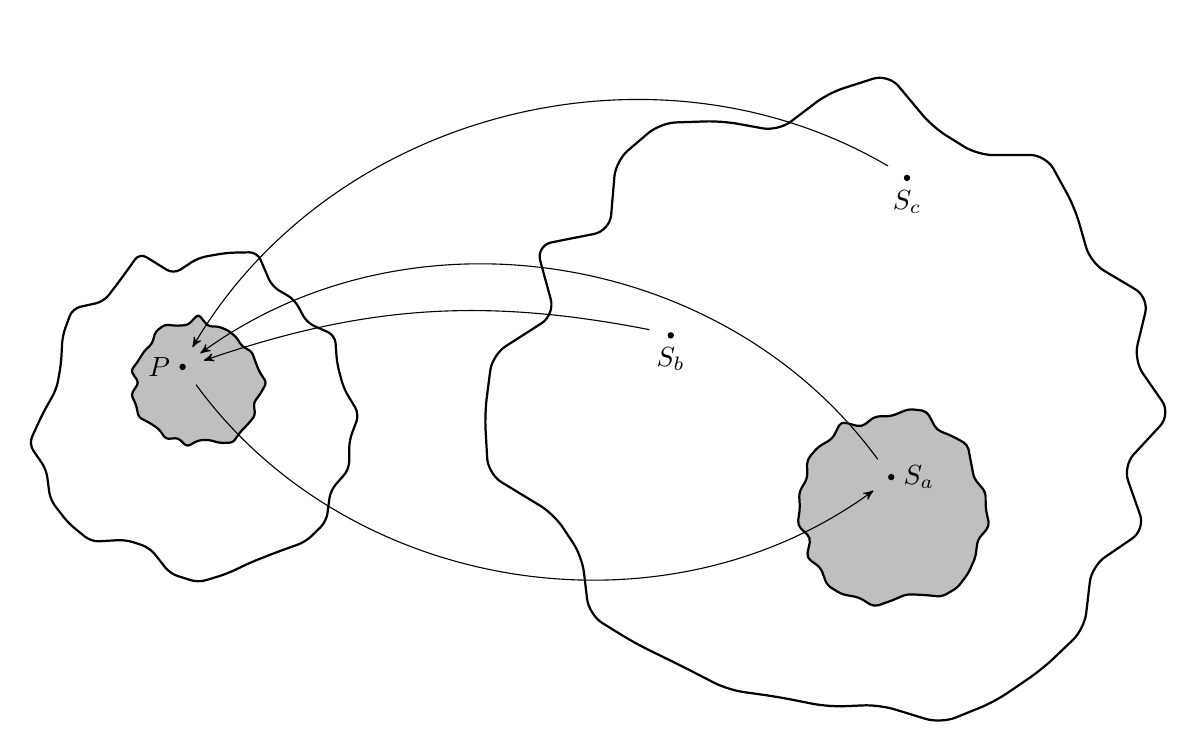
\begin{tikzpicture}
  \coordinate (o) at (0,0) {};
  \coordinate (p) at (-8,0);
  \coordinate (q) at (0.8,-1.2);
  \coordinate (r) at (-8,0.4);
  \draw[rounded corners=2mm,thick] (o) \irregularcircle{4cm}{4mm};
  \draw[rounded corners=1mm, thick] (p) \irregularcircle{2cm}{2mm};
  \draw[rounded corners=0.6mm,thick,fill=gray!50] (q) \irregularcircle{1.2cm}{1.2mm};
  \draw[rounded corners=0.4mm,thick,fill=gray!50] (r) \irregularcircle{0.8cm}{0.8mm};
%  \node (a) at (0.8,-1.2) [] {$\mathcal{M}$};
%  \node (b) at (-8,0.4) [] {$\mathcal{I}$};
%  \node (c) at (0,4) [label=above:$\mathcal{S}$] {};
%  \node (d) at (-8,2) [label=above:$\mathcal{P}$] {};
%  \draw [pil] (q.south west) to [bend left=45] node [] {} (r.south east); 
%  \draw [pilar] (r.north east) to [bend left=45] node [] {} (q.north west);
  \node (P) at (-8.2,0.6) [style={draw,shape=circle,fill=black,scale=0.2},label=left:$P$] {};
  \node (S) at (0.8,-0.8) [style={draw,shape=circle,fill=black,scale=0.2},label=right:$S_a$] {};
  \node (T) at (-2,1) [style={draw,shape=circle,fill=black,scale=0.2},label=below:$S_b$] {};
  \node (U) at (1,3) [style={draw,shape=circle,fill=black,scale=0.2},label=below:$S_c$] {};
  \draw [pil] (S.north west) to [bend right=45] node [] {} (P.north east);
  \draw [pil] (T.north west) to [bend right=15] node [] {} (P.east);
  \draw [pil] (U.north west) to [bend right=45] node [] {} (P.north);
  \draw [pilar] (P.south east) to [bend right=45] node [] {} (S.south west);
\end{tikzpicture}
\end{document}